\documentclass[nonav,sleutel]{beamer}
\usepackage[utf8]{inputenc}
\usepackage[T1]{fontenc}

\title{Politicians and Nobel Prizes}
\date[ISPN '80]{Prof. Dr. Bettina Berendt\\ Knowledge \& the Web 2015-2016}
\author{Katrien Laenen \and Gust Verbruggen \and Ward Schodts}

\usetheme{kuleuvenstijl}

\usepackage{float}
\usepackage{graphicx}
\usepackage{caption}
\usepackage{subcaption}
\graphicspath{ {images/} }

\definecolor{Green7}{RGB}{0, 165, 80}
\definecolor{Red7}{RGB}{200, 8, 21}

\begin{document}

\begin{frame}
\titlepage
\end{frame}


\begin{frame}[noframenumbering]
\frametitle{Outline} 
  \tableofcontents[hideallsubsections
  ]
\end{frame}

\AtBeginSection[]
{
 \begin{frame}<beamer>
 \frametitle{Outline}
 \tableofcontents[hideothersubsections,currentsection]
 \end{frame}
}


\section{Introduction}
\subsection{Some history}
\begin{frame}
\frametitle{Some history}
\framesubtitle{Nobelprizes, what are they?}
\begin{center}


\begin{figure}[H]    
    \begin{subfigure}[b]{0.33\textwidth}
        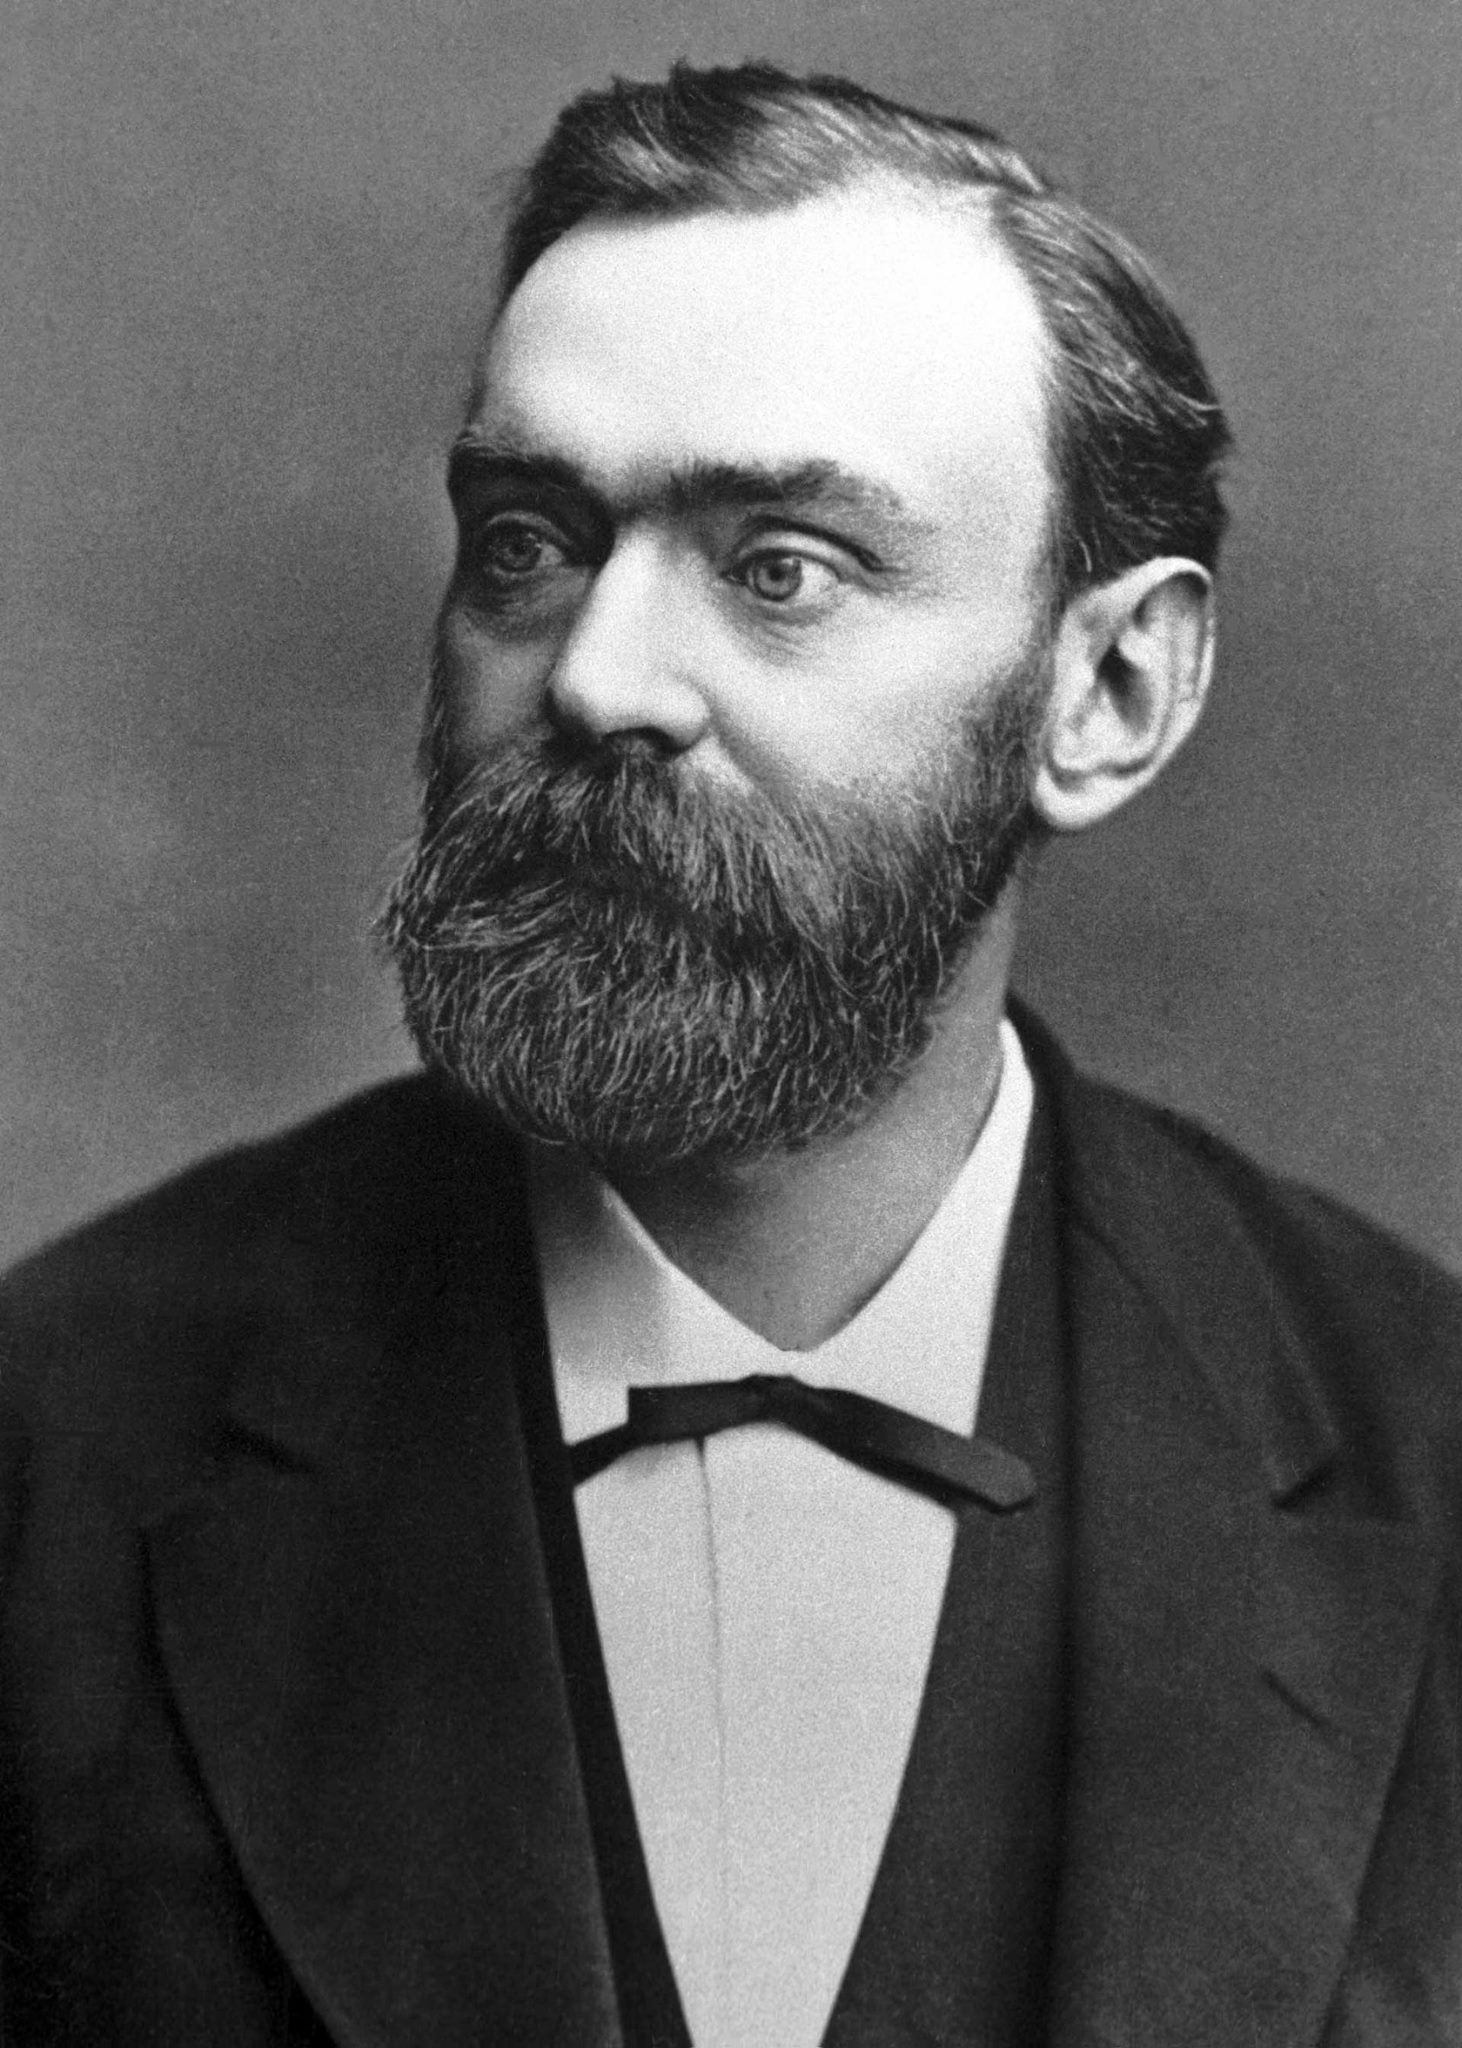
\includegraphics[width=\textwidth]{alfred.jpg}
        \caption{Alfred Nobel}
    \end{subfigure}
    \hspace{2cm}
    \begin{subfigure}[b]{0.33\textwidth}
        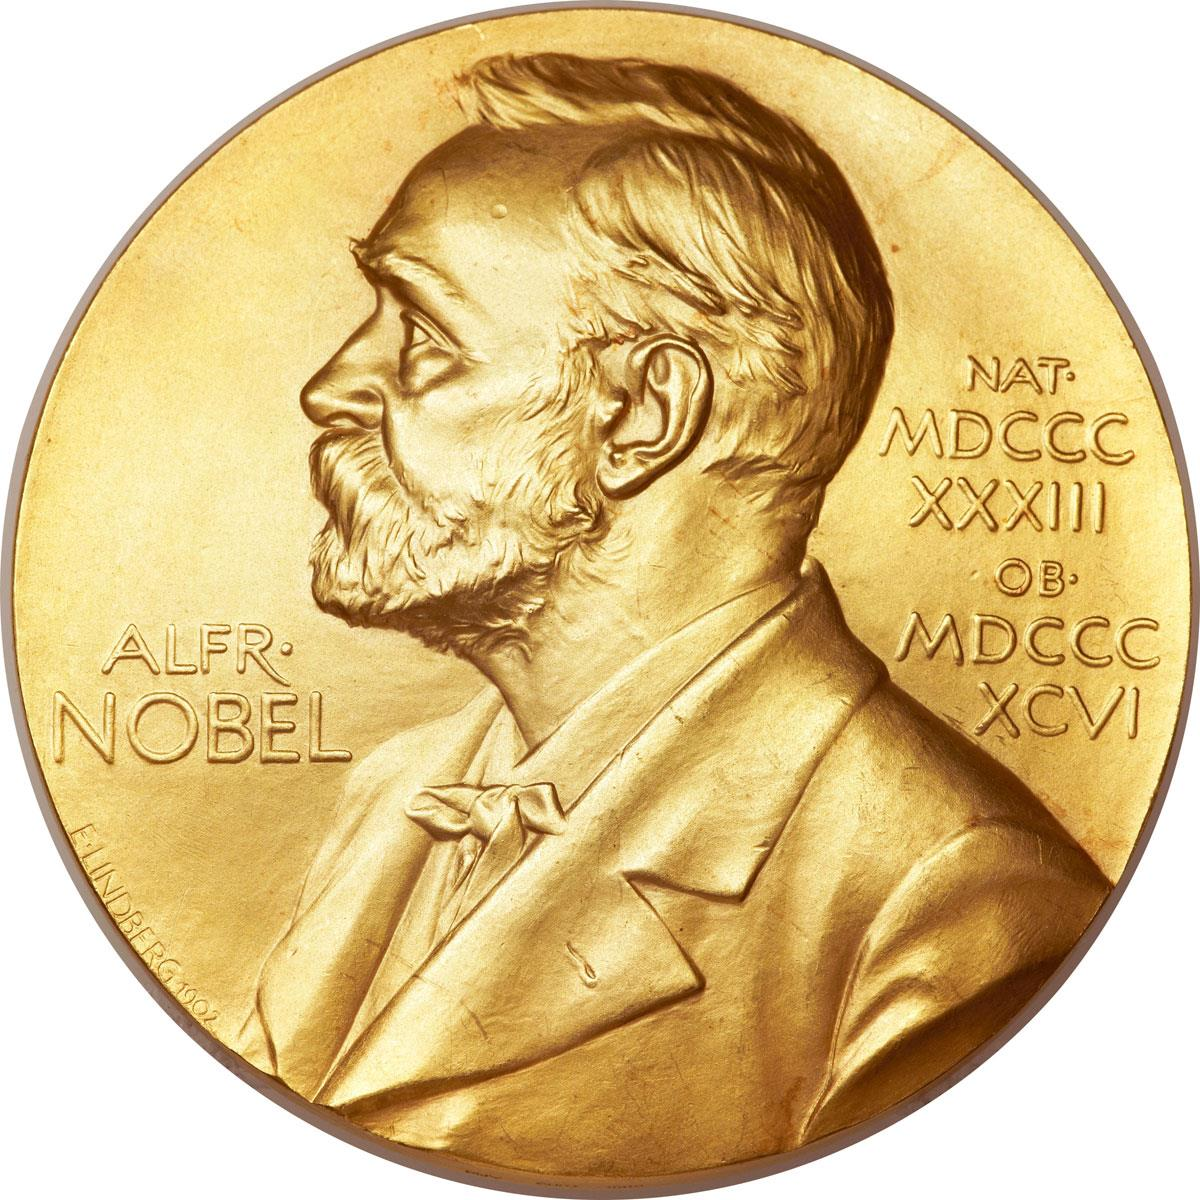
\includegraphics[width=\textwidth]{nobel.jpg}
        \caption{Alfred Nobel}
    \end{subfigure}
\end{figure}
\end{center}
\end{frame}



%%%%%%%%%%%%%%%%%%%%%%%%%%%%%%%%%%%%%%%%%%%%%%%%%%%%%%%%%%%%%%%%%%%%%%%%%%%%%%%%%%%%%%%%%%%%%%%
\subsection{The research question}
\begin{frame}
\frametitle{Our research question} 

\begin{center}
\textit{\Large Which European politicians have a high chance of
receiving a Nobel Prize?}
\end{center}

\end{frame}

\section{Methodology}
\begin{frame}
\frametitle{Methodology}
\framesubtitle{How we will tackle this problem}
\begin{enumerate}
\item<1-> Feature selection: determine features and look for available data
\item<2-> Collecting and combining the data (SPARQL, scraping,...)
\item<3-> Data analysis: learning the model
\item<4-> Interpreting the results
\item<5-> Have a drink
\end{enumerate}
\end{frame}

\section{Data}

\newcounter{featureCounter}
\subsection{Feature selection}
\begin{frame}
\frametitle{Feature selection}
To learn our model, we use the following features\\[.5cm]
\begin{enumerate}
\item<1-> Birth year and -place
\item<2-> Award ranking of alma mater
\item<3-> Work productivity: \# publications $\leftrightarrow$ \# speeches
	\begin{itemize}
		\item[$\rightarrow$] Normalized for each category by dividing by maximum value 
	\end{itemize}
\item<4-> Popularity (likes on Facebook)
	\begin{itemize}
		\item[$\rightarrow$] Also normalized for each category
	\end{itemize}
\setcounter{featureCounter}{\theenumi}
\end{enumerate}
\vspace{.5cm}
\only<5->{
in order to distinguish the class label\\[.5cm]
\begin{enumerate}
\setcounter{enumi}{\thefeatureCounter}
	\item Whether they have won an award
\end{enumerate}
}
\end{frame}

\subsection{Data collection}
\begin{frame}
\frametitle{Data scheme}
\framesubtitle{Where do we get our data?}

\begin{figure}
	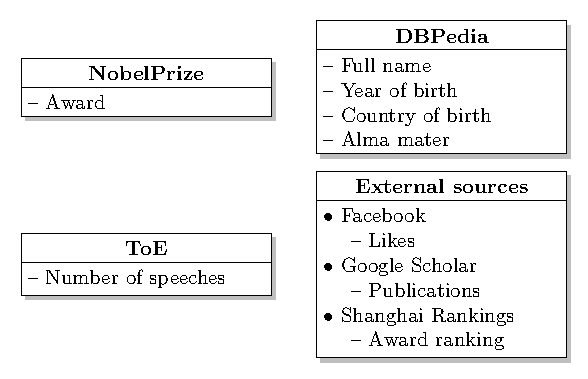
\includegraphics{images/dataschema_original}
\end{figure}

\end{frame}

\begin{frame}
\frametitle{Data scheme}
\framesubtitle{Where do we get our \textbf{\textcolor{Green7}{training}} data?}

\begin{figure}
	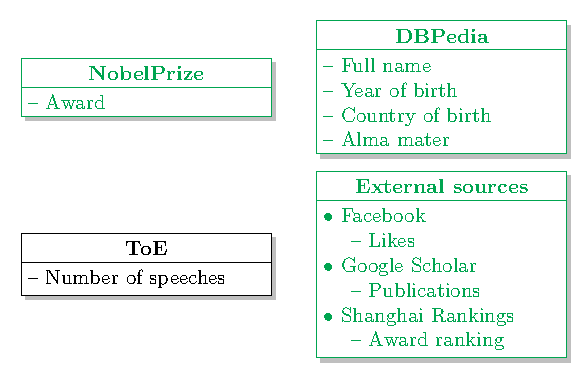
\includegraphics{images/dataschema_training}
\end{figure}

\end{frame}

\begin{frame}
\frametitle{Data scheme}
\framesubtitle{Where do we get our \textbf{\textcolor{Red7}{research}} data?}
\begin{figure}
	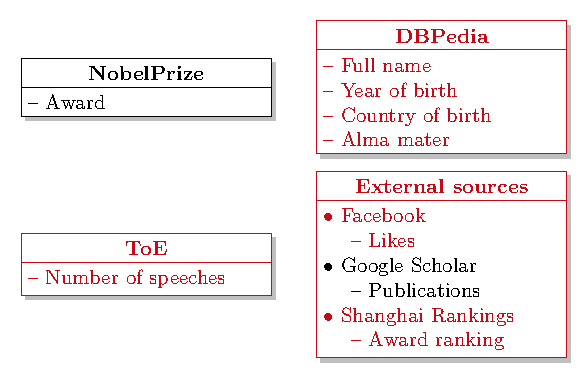
\includegraphics{images/dataschema_research}
\end{figure}
\end{frame}

\begin{frame}
\frametitle{Data scheme}
\framesubtitle{What data do we \textbf{\textcolor{Green7}{already have}}?}
\begin{figure}
	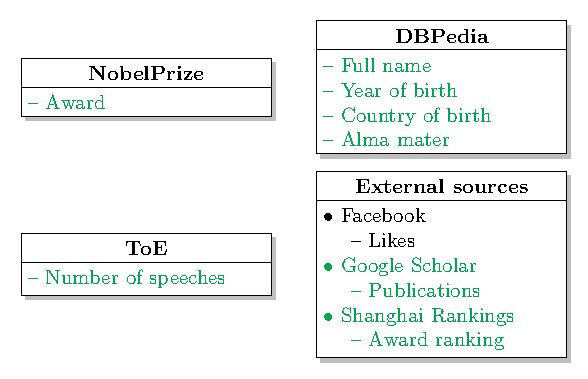
\includegraphics{images/dataschema_done}
\end{figure}
\end{frame}

\section{Analysis}

\subsection{Outlier detection}
\begin{frame}{Outlier detection}
For better analysis, we remove outliers from the data by drawing \textbf{boxplots}.
\begin{figure}
	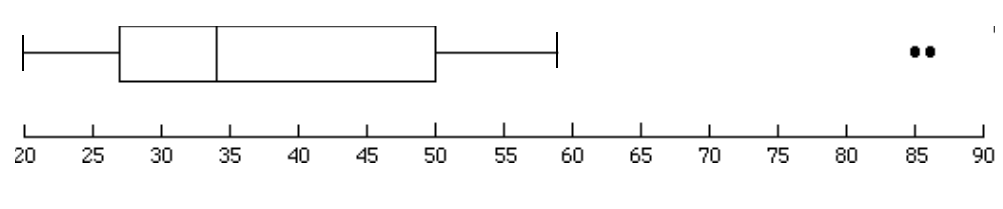
\includegraphics[scale=0.5]{images/boxplot.png}
\end{figure}
\end{frame}


\subsection{Learning the model}

\begin{frame}{Logistic regression}
We need a model that predicts the \emph{probability} of beloning to a class.\\[.5cm]
	\pause
	\begin{itemize}
		\item[$\rightarrow$] \textbf{Multivariate Logistic Regression}
	\end{itemize}
\vspace{.5cm}
Using RapidMiner, such model can be easily learned and applied. 
\end{frame}

\section{Results}

\begin{frame}{Results}
... yet to be tested!\\[.5cm]
	
\end{frame}

\section{Conclusion}

\begin{frame}{Difficulties}
\begin{itemize}
	\item<1-> Few positive examples compared to negative examples
		\begin{itemize}
			\item[$\rightarrow$] Sampling?
		\end{itemize}
	\item<2-> Data that's not already linked is hard to link
		\begin{itemize}
			\item[$\rightarrow$] E.g. fuzzy matching of university names
		\end{itemize}
	\item<3-> Google Scholar is being lame
		\begin{itemize}
			\item[$\rightarrow$] Blocks us from scraping
		\end{itemize}
\end{itemize}
\end{frame}

\begin{frame}
\begin{center}
\Large{Thanks for listening}\\
Any questions?
\end{center}

\end{frame}

\end{document}